\documentclass{beamer}
\usepackage[T1]{fontenc}
\usepackage[utf8]{inputenc}
\usepackage{lmodern}
\usepackage[english]{babel}

\usepackage{verbatim}
\usepackage{mathtools}
\usepackage{stmaryrd}


\usepackage{geometry}
\usepackage{setspace}

\usepackage{latex/agda}
\usepackage{unicode-math}
\setmathfont{XITS Math}

\usepackage{newunicodechar}
\newunicodechar{→}{\ensuremath{\mathnormal\to}}
\newunicodechar{ℕ}{\ensuremath{\mathnormal\bN}}

\usepackage{xcolor}
\usepackage[normalem]{ulem}%per barrare parole
\usepackage{soul} %barrare numeri
% \usepackage{booktabs}%per tabelle
\usepackage{amsmath} %leqno mette elenchi in align a sx
\usepackage{amssymb}
% \usepackage{enumitem} %personalizza gli elenchi
% \usepackage{amsthm} %teoremi e definizioni
\usepackage{tikz-cd}
\usepackage{adjustbox}

\usepackage{multirow}%più righe nella stessa cella in tabella
\usepackage{multicol}
\usepackage{caption}
\usepackage{bussproofs}

\usetheme{Antibes}
\usecolortheme{beaver}
\useinnertheme{rounded}
\useoutertheme{infolines}

% \titlegraphic{
\includegraphics[width=25mm]{pics/aisec.png}}
\title{On the syntax and semantics of voice assistants in autonomous vehicles}
\author{Warrick Macmillan}
\date{$6^{th}$ May 2022}



\begin{document}

\begin{frame}
  \titlepage
\end{frame}

\section{Overview}


% \subsection{Quick Recapitulation}

% \begin{frame}
% \begin{code}%
\>[0]\<%
\\
\>[0]\AgdaKeyword{data}\AgdaSpace{}%
\AgdaDatatype{Nat}\AgdaSpace{}%
\AgdaSymbol{:}\AgdaSpace{}%
\AgdaPrimitive{Set}\AgdaSpace{}%
\AgdaKeyword{where}\<%
\\
\>[0][@{}l@{\AgdaIndent{0}}]%
\>[2]\AgdaInductiveConstructor{zero}\AgdaSpace{}%
\AgdaSymbol{:}\AgdaSpace{}%
\AgdaDatatype{Nat}\<%
\\
%
\>[2]\AgdaInductiveConstructor{suc}\AgdaSpace{}%
\AgdaSymbol{:}\AgdaSpace{}%
\AgdaDatatype{Nat}\AgdaSpace{}%
\AgdaSymbol{->}\AgdaSpace{}%
\AgdaDatatype{Nat}\<%
\\
\>[0]\<%
\end{code}

% \end{frame}

% \begin{frame}
% \begin{code}%
\>[0]\<%
\\
\>[0]\AgdaKeyword{open}\AgdaSpace{}%
\AgdaKeyword{import}\AgdaSpace{}%
\AgdaModule{F}\<%
\\
%
\\[\AgdaEmptyExtraSkip]%
\>[0]\AgdaFunction{plus}\AgdaSpace{}%
\AgdaSymbol{:}\AgdaSpace{}%
\AgdaDatatype{Nat}\AgdaSpace{}%
\AgdaSymbol{→}\AgdaSpace{}%
\AgdaDatatype{Nat}\AgdaSpace{}%
\AgdaSymbol{→}\AgdaSpace{}%
\AgdaDatatype{Nat}\<%
\\
\>[0]\AgdaFunction{plus}\AgdaSpace{}%
\AgdaInductiveConstructor{zero}\AgdaSpace{}%
\AgdaBound{b}\AgdaSpace{}%
\AgdaSymbol{=}\AgdaSpace{}%
\AgdaBound{b}\<%
\\
\>[0]\AgdaFunction{plus}\AgdaSpace{}%
\AgdaSymbol{(}\AgdaInductiveConstructor{suc}\AgdaSpace{}%
\AgdaBound{a}\AgdaSymbol{)}\AgdaSpace{}%
\AgdaBound{b}\AgdaSpace{}%
\AgdaSymbol{=}\AgdaSpace{}%
\AgdaInductiveConstructor{suc}\AgdaSpace{}%
\AgdaSymbol{(}\AgdaFunction{plus}\AgdaSpace{}%
\AgdaBound{a}\AgdaSpace{}%
\AgdaBound{b}\AgdaSymbol{)}\<%
\\
\>[0]\<%
\end{code}

% \end{frame}



\begin{frame}
\frametitle{Motivation}

\begin{exampleblock}{}

  ``Go to the grocery store after the next exit, and then go to fuel station,
but stop by the fire hydrant so I can take a picture of that crazy sign,
first.''

\end{exampleblock}
\pause
\begin{figure}
\hspace*{-3mm}%
\centering
   \pause
   
\includegraphics[width=1.5cm]{pics/hydrant.png}
   \pause
   
\includegraphics[width=3cm]{pics/crazy.jpg}
   % 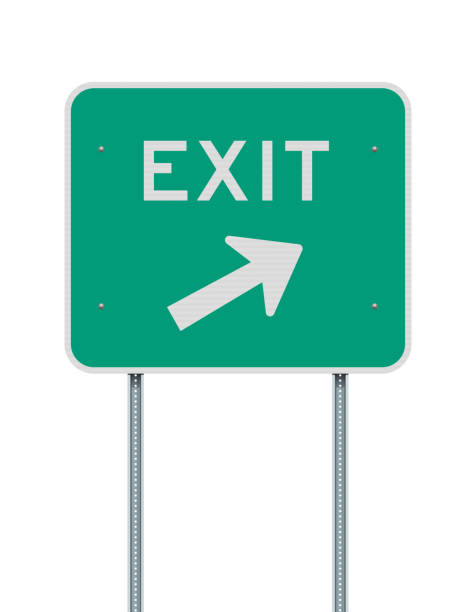
\includegraphics[width=2cm]{pics/exit.jpg}
   % 
\includegraphics[width=3cm]{pics/shop.jpeg}
\end{figure}
\pause
\begin{figure}
\hspace*{-3mm}%
\centering
   % 
\includegraphics[width=1.5cm]{pics/hydrant.png}
   % 
\includegraphics[width=3cm]{pics/crazy.jpg}
   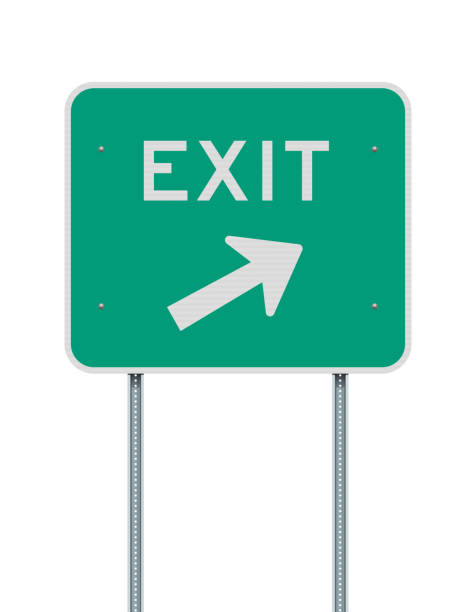
\includegraphics[width=2cm]{pics/exit.jpg}
   \pause
   
\includegraphics[width=3cm]{pics/shop.jpeg}
   \pause
   
\includegraphics[width=3cm]{pics/charge.jpg}
\end{figure}
  
\end{frame}

\begin{frame}
\frametitle{Ambiguities}

\begin{center}
\begin{minipage}{4cm}
\begin{alertblock}{}
``Go into the other lane''
\end{alertblock}
\end{minipage}
\end{center}
\pause
\begin{figure}
\hspace*{-3mm}%
\centering
    % \includegraphics[width=4cm,angle=45]{Ques}
    % \includegraphics[angle=45,width=4cm]{Ques}
   
\includegraphics[width=4cm]{pics/singleLane.jpg}
   \pause
   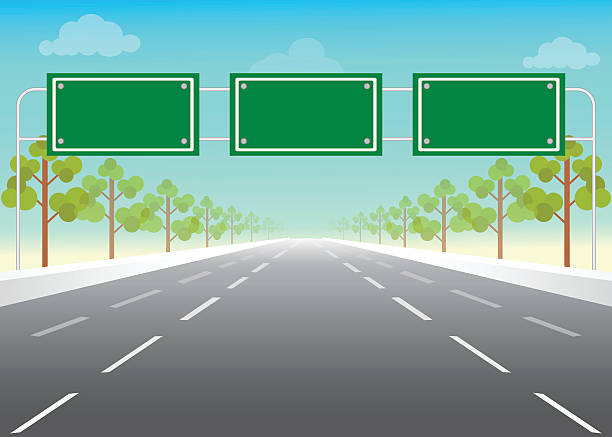
\includegraphics[width=6cm]{pics/multipleLane.jpg}
\end{figure}
  
\end{frame}

\begin{frame}

\frametitle{Ambiguities (cont.)}

\begin{center}
\begin{minipage}{6cm}
\begin{alertblock}{}
``Drive to the person with the dog''
\end{alertblock}
\end{minipage}
\end{center}

\pause
\begin{figure}
\hspace*{-3mm}%
\centering
   
\includegraphics[width=5cm]{pics/personDog.png}
   \pause
   
\includegraphics[width=5cm]{pics/dogCar.png}
\end{figure}
  
\end{frame}

\begin{frame}
\frametitle{Simplified Autonomous Vehicle}
\begin{figure}
\centering
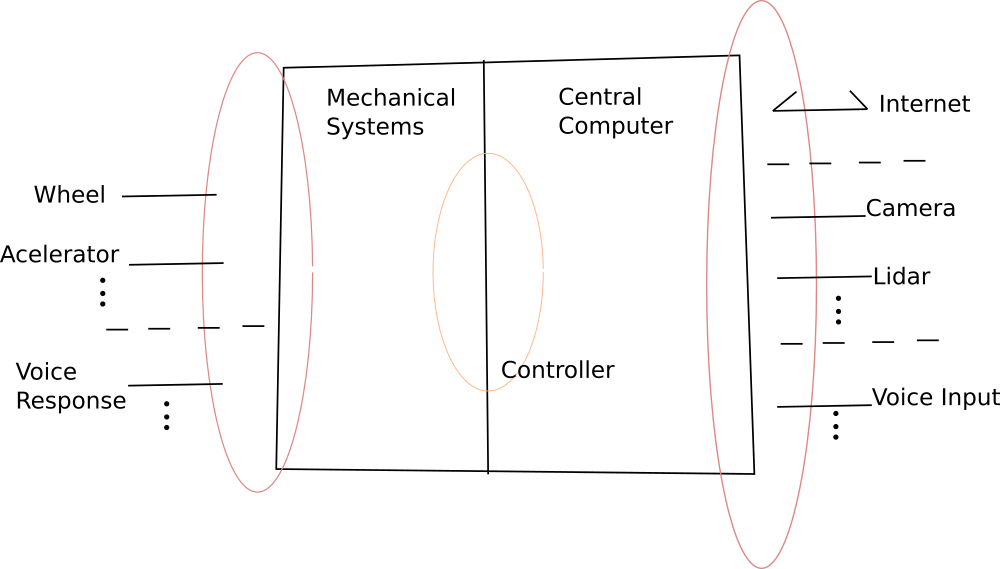
\includegraphics[width=100mm]{pics/selfDriving.png}
\caption{Self-driving car}\label{fig:A1}
\end{figure}

\end{frame}

\begin{frame}
\frametitle{Path}
\begin{figure}
\centering
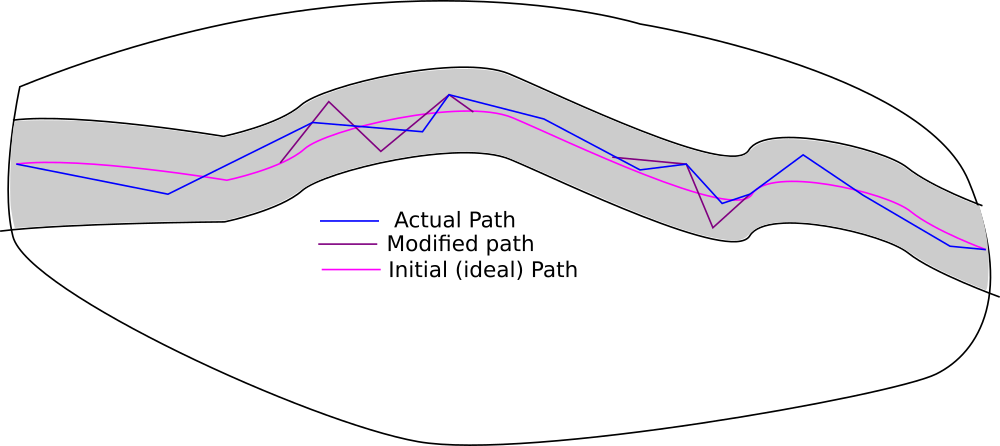
\includegraphics[width=100mm]{pics/diagramTrial1.png}
\caption{Initial, modified, and actual paths/routes}\label{fig:A2}
\end{figure}

\end{frame}

\begin{frame}
\begin{block}{Mathematically Ideal Property}
  $\forall u \in \text{Utt}\; \exists r \in \text{Routes}$
  such that $\forall r' \in \text{Routes}\; d(u,r) \leq d(u,r')$
\end{block}
\pause
\begin{exampleblock}{}
where $d$ is some hypothetical metric which should depend on
\begin{itemize}
\item Cost
\item Safety
\item Legality
\item Adversaries
\end{itemize}
\end{exampleblock}

\pause
\begin{exampleblock}{}
and where
\begin{itemize}
\item The set of utterances is a set of strings over a standard alphabet
\item The set of routes is some discretized set of paths in Euclidean 2-space
\end{itemize}
subject to constraints on the sets imposed by, for example
\begin{itemize}
\item grammars in the case of strings
\item or physical objects in the case of paths in Euclidean space
\end{itemize}
\end{exampleblock}



% \begin{itemize}
% \item Functional Programming languages : GF (Grammatical Framework), Haskell, Theorem Provers (Agda, Coq, ...)
% \item Verification for Robotics Systems :  Temporal logic (mostly at the syntactic level, for now)
% \item Natural Language Processing : Semantic Parsing, Controlled Natural Languages
% \end{enumerate}



\end{frame}


\begin{frame}[fragile]
\begin{figure}
\centering

% https://tikzcd.yichuanshen.de/#N4Igdg9gJgpgziAXAbVABwnAlgFyxMJZABgBpiBdUkANwEMAbAVxiRAB12cYAPHYAMpYwAcwYwABAFEedALZpxAXxBLS6TLnyEUZAIxVajFm1XqQGbHgJEA7KQPV6zVohBmNV7UQBM5Q84mbpzcfIIwOBIQAGbSsgricCpqnlo2KAAs-k7GrhxcvPxCouISAAoAThBoMBU4AJ7J5pZpOsgAbNlGLmwhhcAAshF0aFU1dY0eFprWbWQ+Abm9BWEAqmC4EgAq8DhNqbO+pAs5PcEr-JXVtQ0AtABGdHAwUNu7+9Ne6chZJ91B+VC-AG0BgDAkAGEABYwADGAGthCIPi1DihOn9Ank+mEAJJgbgVOiwvA0SRbGEQCowOTlKpkioombeFB6Y6LM7uFKfVpHADMHIBU1RLOQfPZpyF3JF3yyAsleWFzO+AFYJf9FdLlW1OvKNaYtV82myMoLNc1tUQABykU0Kg2GF4ieBEUDRKpyJBskA4CBIHzc90QT2IPRkH1+0N6QMer1+CNevkx4NerIJ0Mq5MhvSddN6ewgBh0e5gsqWtzCbCwED285A4AAMSYYBJ2kYdIgIiJcjkSIkAihWGie1UFCUQA
\adjustbox{scale=2,center}{%
\begin{tikzcd}
\text{Single Example} &                                                                       & \text{Set of Examples}     &               & \text{Single Property} &               & \text{Metaproperty}               &    &    \\
{} \arrow[rrrrrrr]    &                                                                       &                            &               &                        &               &                                   & {} &    \\
\text{Unit Test}      & {} \arrow[rd]                                                         & \text{Property-based Test} & {} \arrow[rd] & \text{Model Checking}  & {} \arrow[rd] & \text{Interactive Theorem Prover} &    &    \\
                      &                                                                       & {}                         &               & {}                     &               & {}                                &    &    \\
                      & {} \arrow[rrrrrrr, "\text{Functional Programming Shift}" description] &                            &               &                        &               &                                   &    & {}
                      }
\end{tikzcd}
\end{figure}

\end{frame}

\begin{frame}
\frametitle{Ambiguities (cont.)}
\end{frame}

% \begin{frame}
% \frametitle{Big Picture}

% \begin{exampleblock}{Manifold Ideas}
% This project contains bits and pieces of :
% \end{exampleblock}

% \begin{enumerate}
% \item Functional Programming languages : GF (Grammatical Framework), Haskell, Theorem Provers (Agda, Coq, ...)
% \item Verification for Robotics Systems :  Temporal logic (mostly at the syntactic level, for now)
% \item Natural Language Processing : Semantic Parsing, Controlled Natural Languages
% \end{enumerate}
% \end{frame}



\begin{frame}

\begin{exampleblock}{}
This project is quite multifaceted, still in a somewhat primordial state (and therefore may be taken in many directions).
\end{exampleblock}

\begin{block}{}
Goal : Design a controlled natural language which is 
\end{block}

\begin{itemize}
\item Suitable as an ``approximation'' for a voice assistant for an autonomous vehicle
\item Has a well defined semantics in temporal logic
\item Seeking to balance breadth and depth of our system
\end{itemize}

\end{frame}

\begin{frame}

\frametitle{Trade-offs}

\begin{itemize}
\item Breadth : Wide coverage, usable by non-experts (where ML comes in)
\item Depth   : Well-behaved, verifiable (where FP comes in)
\end{itemize}

\end{frame}

\begin{frame}
\frametitle{Ideal Pipeline}

\begin{equation} % \label{eq1}
\begin{split}
\text{Utterance} & \xrightarrow{\mathit{Speech\ Recognizer}} \text{String}\\
 & \xrightarrow{\mathit{Canonicalization_{BERT}}} \text{String}\\
 & \xrightarrow{\mathit{Parsing\ (GF)}} \text{Abstract Syntax Tree (NL)}\\
 & \xrightarrow{\llbracket - \rrbracket_{Haskell}} \text{Abstract Syntax Tree (LTL)}\\
 & \xrightarrow{\vDash} \text{Verifiable Path}
\end{split}
\end{equation} 
\end{frame}

\begin{frame}
\frametitle{What we have so far...}

\begin{equation} % \label{eq1}
\begin{split}
\text{String} & \xrightarrow{\mathit{Parsing\ (GF)}} \text{Abstract Syntax Tree (NL)}\\
 & \xrightarrow{\llbracket - \rrbracket_{Haskell}} \text{Abstract Syntax Tree (LTL)}\\
 & \xrightarrow{\vDash}_{Agda} \text{``Standard Semantics''}
\end{split}
\end{equation} 
\end{frame}


\begin{frame}[fragile]
\frametitle{Example AST}
``go to the store and turn left'' $\mapsto$
\begin{verbatim}
CompoundCommand
    * And
      BasePosCommand
        * SimpleCom
            * ModAction
                * Go
                  MkAdvPh
                    * To
                      WhichObject
                        * The
                          Store
          SimpleCom
            * ModAction
                * Turn
                  WherePhrase (Left)
\end{verbatim}
\end{frame}

\begin{frame}[fragile]
\frametitle{Example Cont..}
${\llbracket  \text{``go to the store and turn left . Finish .''}_{AST} \rrbracket_{Haskell}}$
\begin{verbatim}
F
  (Meet
    (Atom "the_store") 
    (X 
      (Meet 
        (Atom "left") 
        (G (Atom "FINISHED")))))
\end{verbatim}

\begin{exampleblock}{Interpretation}
  
Eventually be in a state where you are at the store. Directly after, you are in
a state where you are left. From thereon, you are forever finished.

\end{exampleblock}
\end{frame}


\begin{frame}
\frametitle{Functional Programming}
\begin{block}{}
Types, and type-checking is a fundamental way to seperate the process of
programming into two phases
\begin{itemize}
\item Static  : Specification, Types 
\item Dynamic : Implentation, Programs 
\end{itemize}
\end{block}

% \begin{exampleblock}{}
\begin{itemize}
\item Correct-by-construction mentality - ``verification technique''
\item Constraints are baked into user-defined types.
\item Specification guides implementation. Functional
  programmers spend almost all their time thinking about types.
\item Focus energy on high-level (abstract) details
\item It is convenient to implement programming languages
(i.e. write interpreters and compilers)
\end{itemize}
% \end{exampleblock}
\end{frame}

\begin{frame}

\frametitle{Grammatical Framework}

\begin{itemize}
\item Functional programming language
\item Implementing natural language parsers and linearizes
\item Separation of abstract syntax and concrete syntax.
\item Intended for translation, multilingual support
\item One designs a grammar, Parallel Multiple CFGs (PMCFG)
\item Chomsky Hierarchy : $\text{CFG} < \text{PMCFG} < \text{Context Sensitive Grammar}$
\item Standard Libarary : Resource Grammar Library (RGL)
\item Embedding in Haskell : Portable Grammar Format (PGF)
\end{itemize}

\end{frame}

\begin{frame}[fragile]
\frametitle{GF Example}

BNFC (traditional treatment of fixity)

\begin{verbatim}
Lam. Exp  ::= "\\" [PTele] "->" Exp ;
App. Exp2 ::= Exp2 Exp3 ;
\end{verbatim}

Abstract :

\begin{verbatim}
fun
  Lam : [Tele] -> Exp -> Exp ;
  App : Exp -> Exp -> Exp ;
\end{verbatim}

Concrete :

\begin{verbatim}
lin
  Lam pt e = mkPrec 0 ("\\" ++ pt ++ "->" ++ usePrec 0 e) ;
  App = infixl 2 "" ;
\end{verbatim}
\end{frame}


\begin{frame}
\frametitle{Haskell and Agda}

\begin{exampleblock}{Haskell}
\begin{itemize}
\item One of the main FP languages - deep ties in Scotland and Sweden
\item GADTs and pattern matching make for first-class tree transformations
\item Defining and reasoning about logics and programming languages
\end{itemize}
\end{exampleblock}

\begin{exampleblock}{Agda}
\begin{itemize}
\item ``Dependently typed Haskell''
\item Interactive Theorem Prover
\item Programs as proofs, propositions as types
\end{itemize}

\end{exampleblock}
\end{frame}

\begin{frame}
\frametitle{Linear Temporal Logic}

\begin{itemize}
\item Modal logic (temporal modality)
\item Allows one to reason about sequential actions
\item Verification for robotics systems
\item Objective in reinforcement learning
\item Other temporal logics (Signal TL, Computation Tree Logic, ...)
\item Decidable 
\end{itemize}

\begin{block}{Complexity (and expressivity)}
$\text{Propositional Logic} < \text{Temporal Logic} <_{undecidable} \text{First Order Logic}$
\end{block}

\begin{exampleblock}{Temporal Operators}
\begin{itemize}
\item $X \phi$ : in the next state, phi holds
\item $\diamond \phi$ : exists a future state such that $\phi$ holds ($F \phi$)
\item $\square \phi$ : $\phi$ holds for every future state ($G \phi$)
\end{itemize}
\end{exampleblock}

\end{frame}

\begin{frame}
\frametitle{Where does ML come in?}

\begin{exampleblock}{Language Models}
\begin{itemize}
\item Foundation models - future of NLP?
\item BERT, GPT3, ...
\item Pretrain and then fine-tune
\end{itemize}
\end{exampleblock}

\begin{block}{Ingredients}
\begin{itemize}
\item Semantic Parser : NL Utterance -> Formal Language form
\item Touchdown Data Set : ~13000 sequences
\item Few-shot semantic parsers paper (Microsoft Research) - open source Pytorch code
\end{itemize}
\end{block}

\begin{alertblock}{Idea}
Integrate their technique and code with our parser and dataset
\end{alertblock}

\end{frame}


\begin{frame}
\frametitle{}
\begin{figure}
\hspace*{-3mm}%
   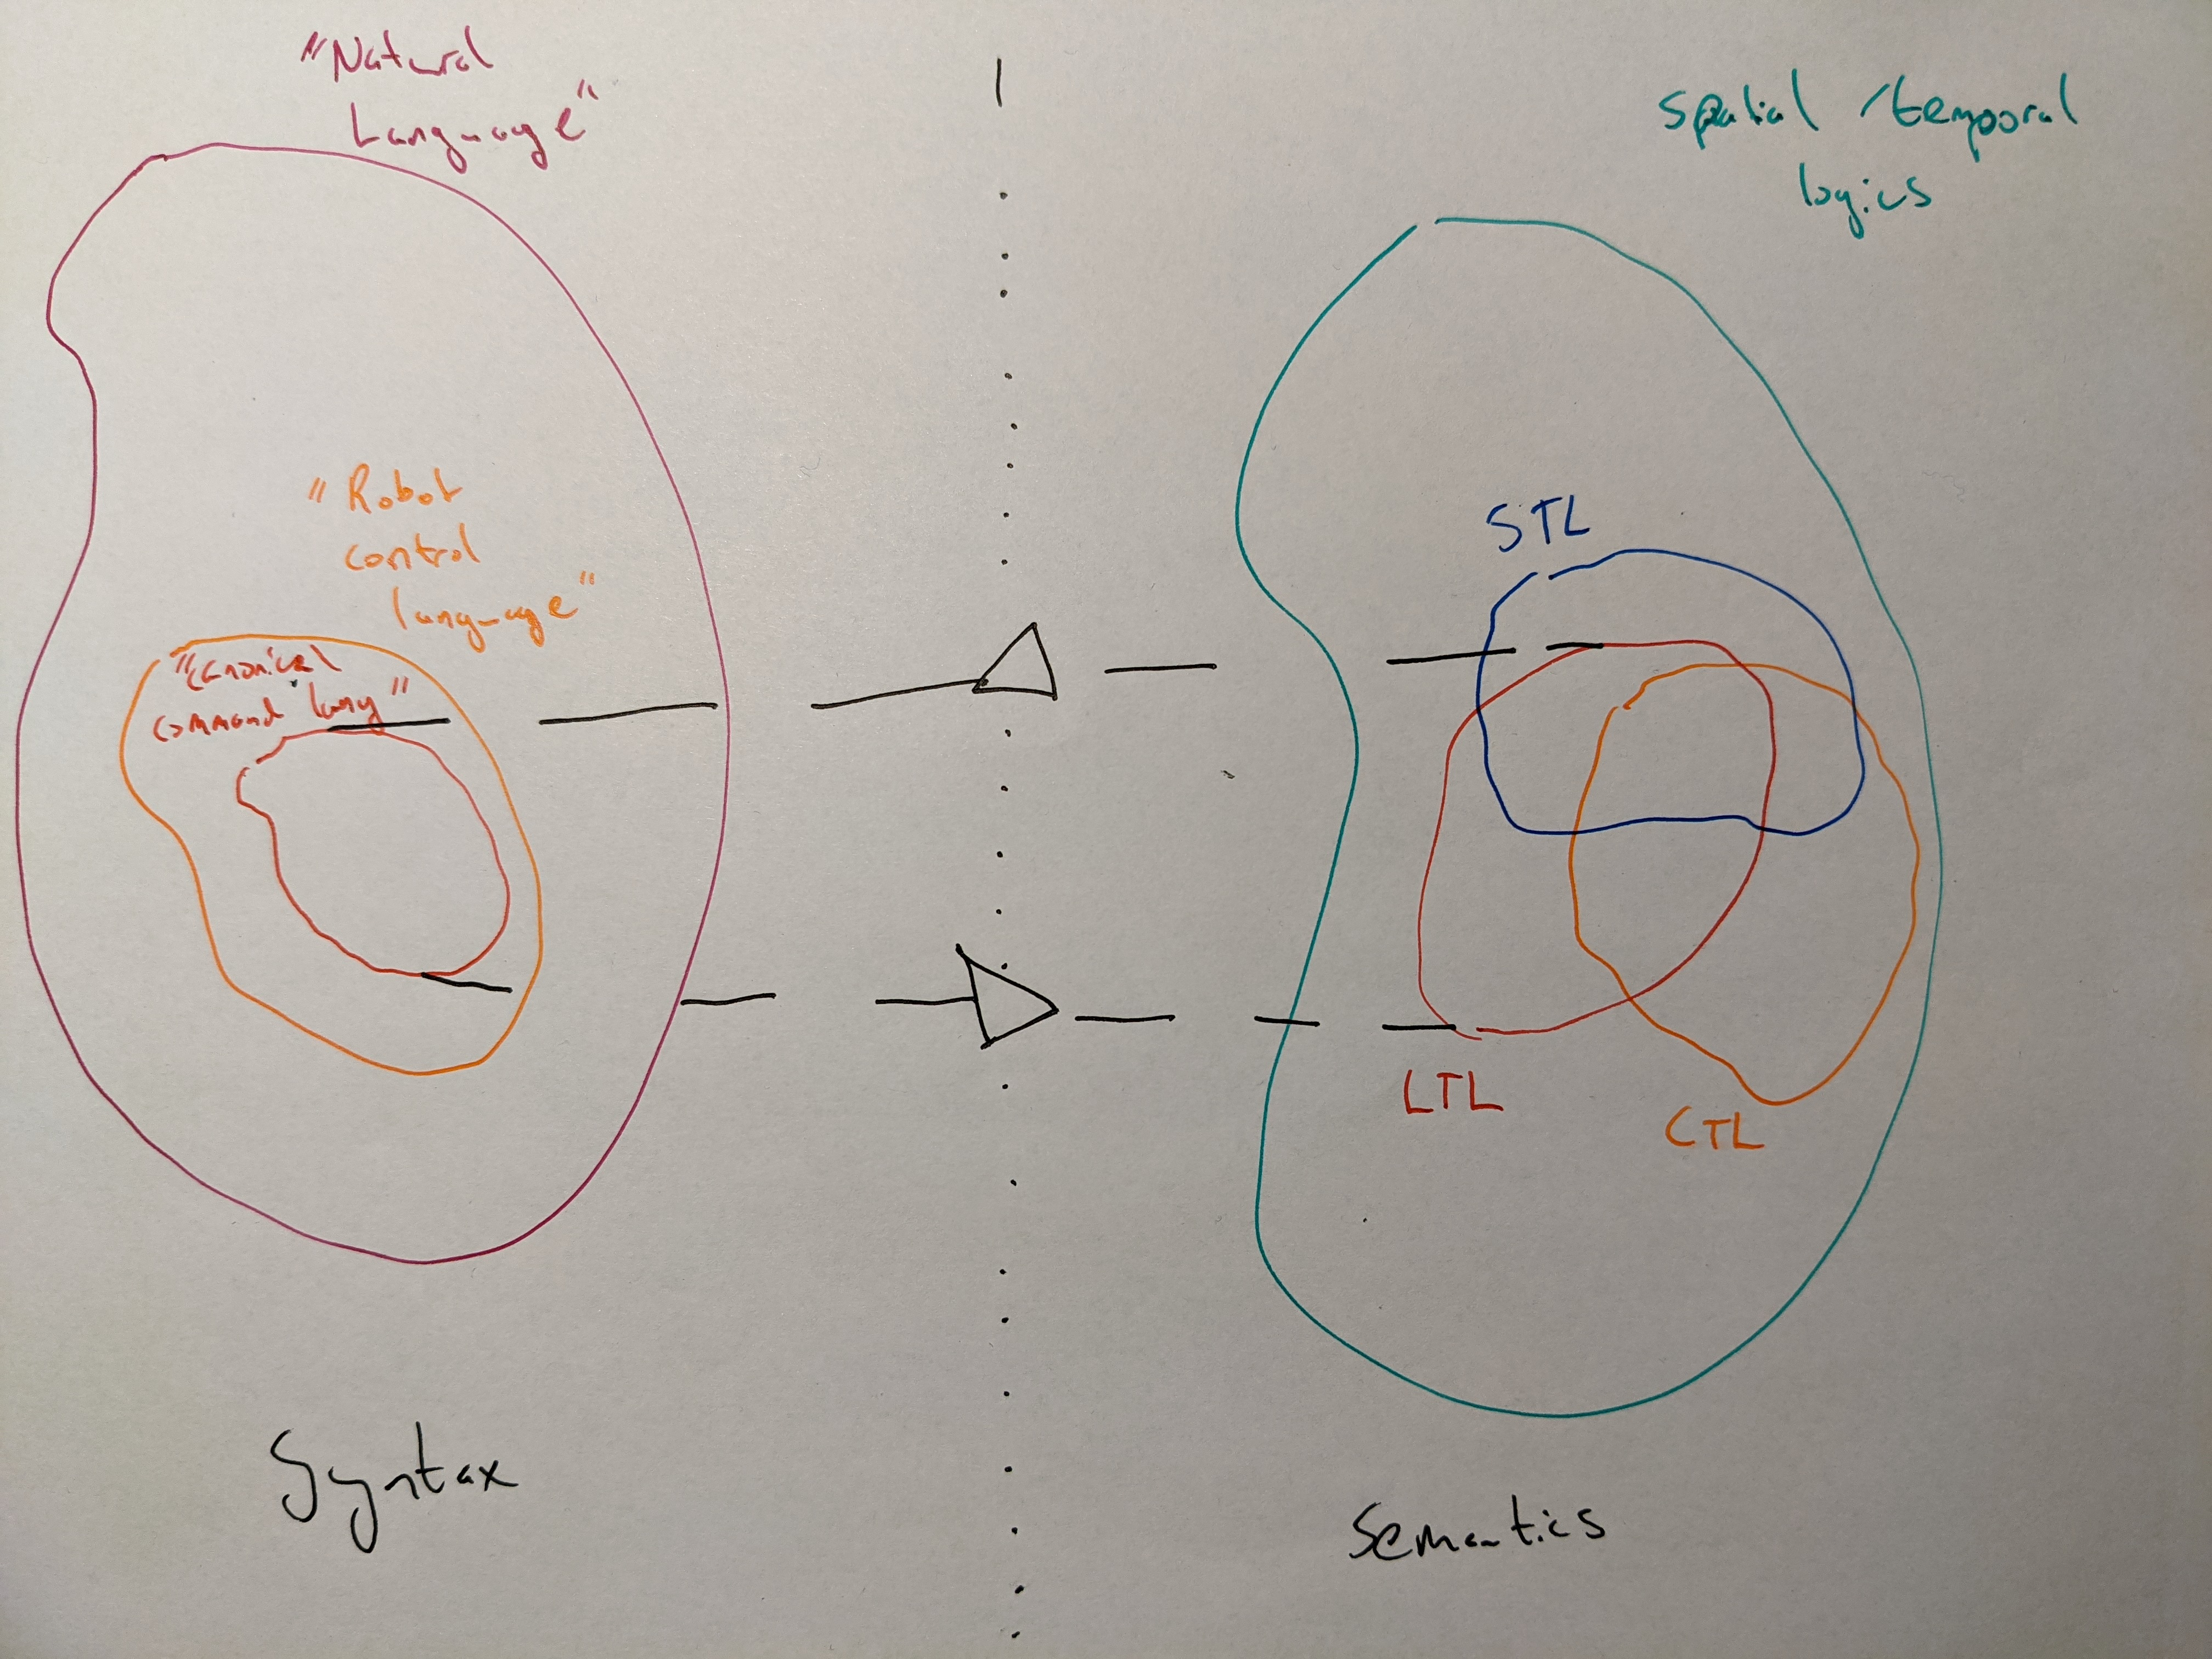
\includegraphics[width= \paperwidth]{pics/one.jpg}
\end{figure}
\end{frame}

\begin{frame}
\frametitle{}
\begin{figure}
\hspace*{-3mm}%
   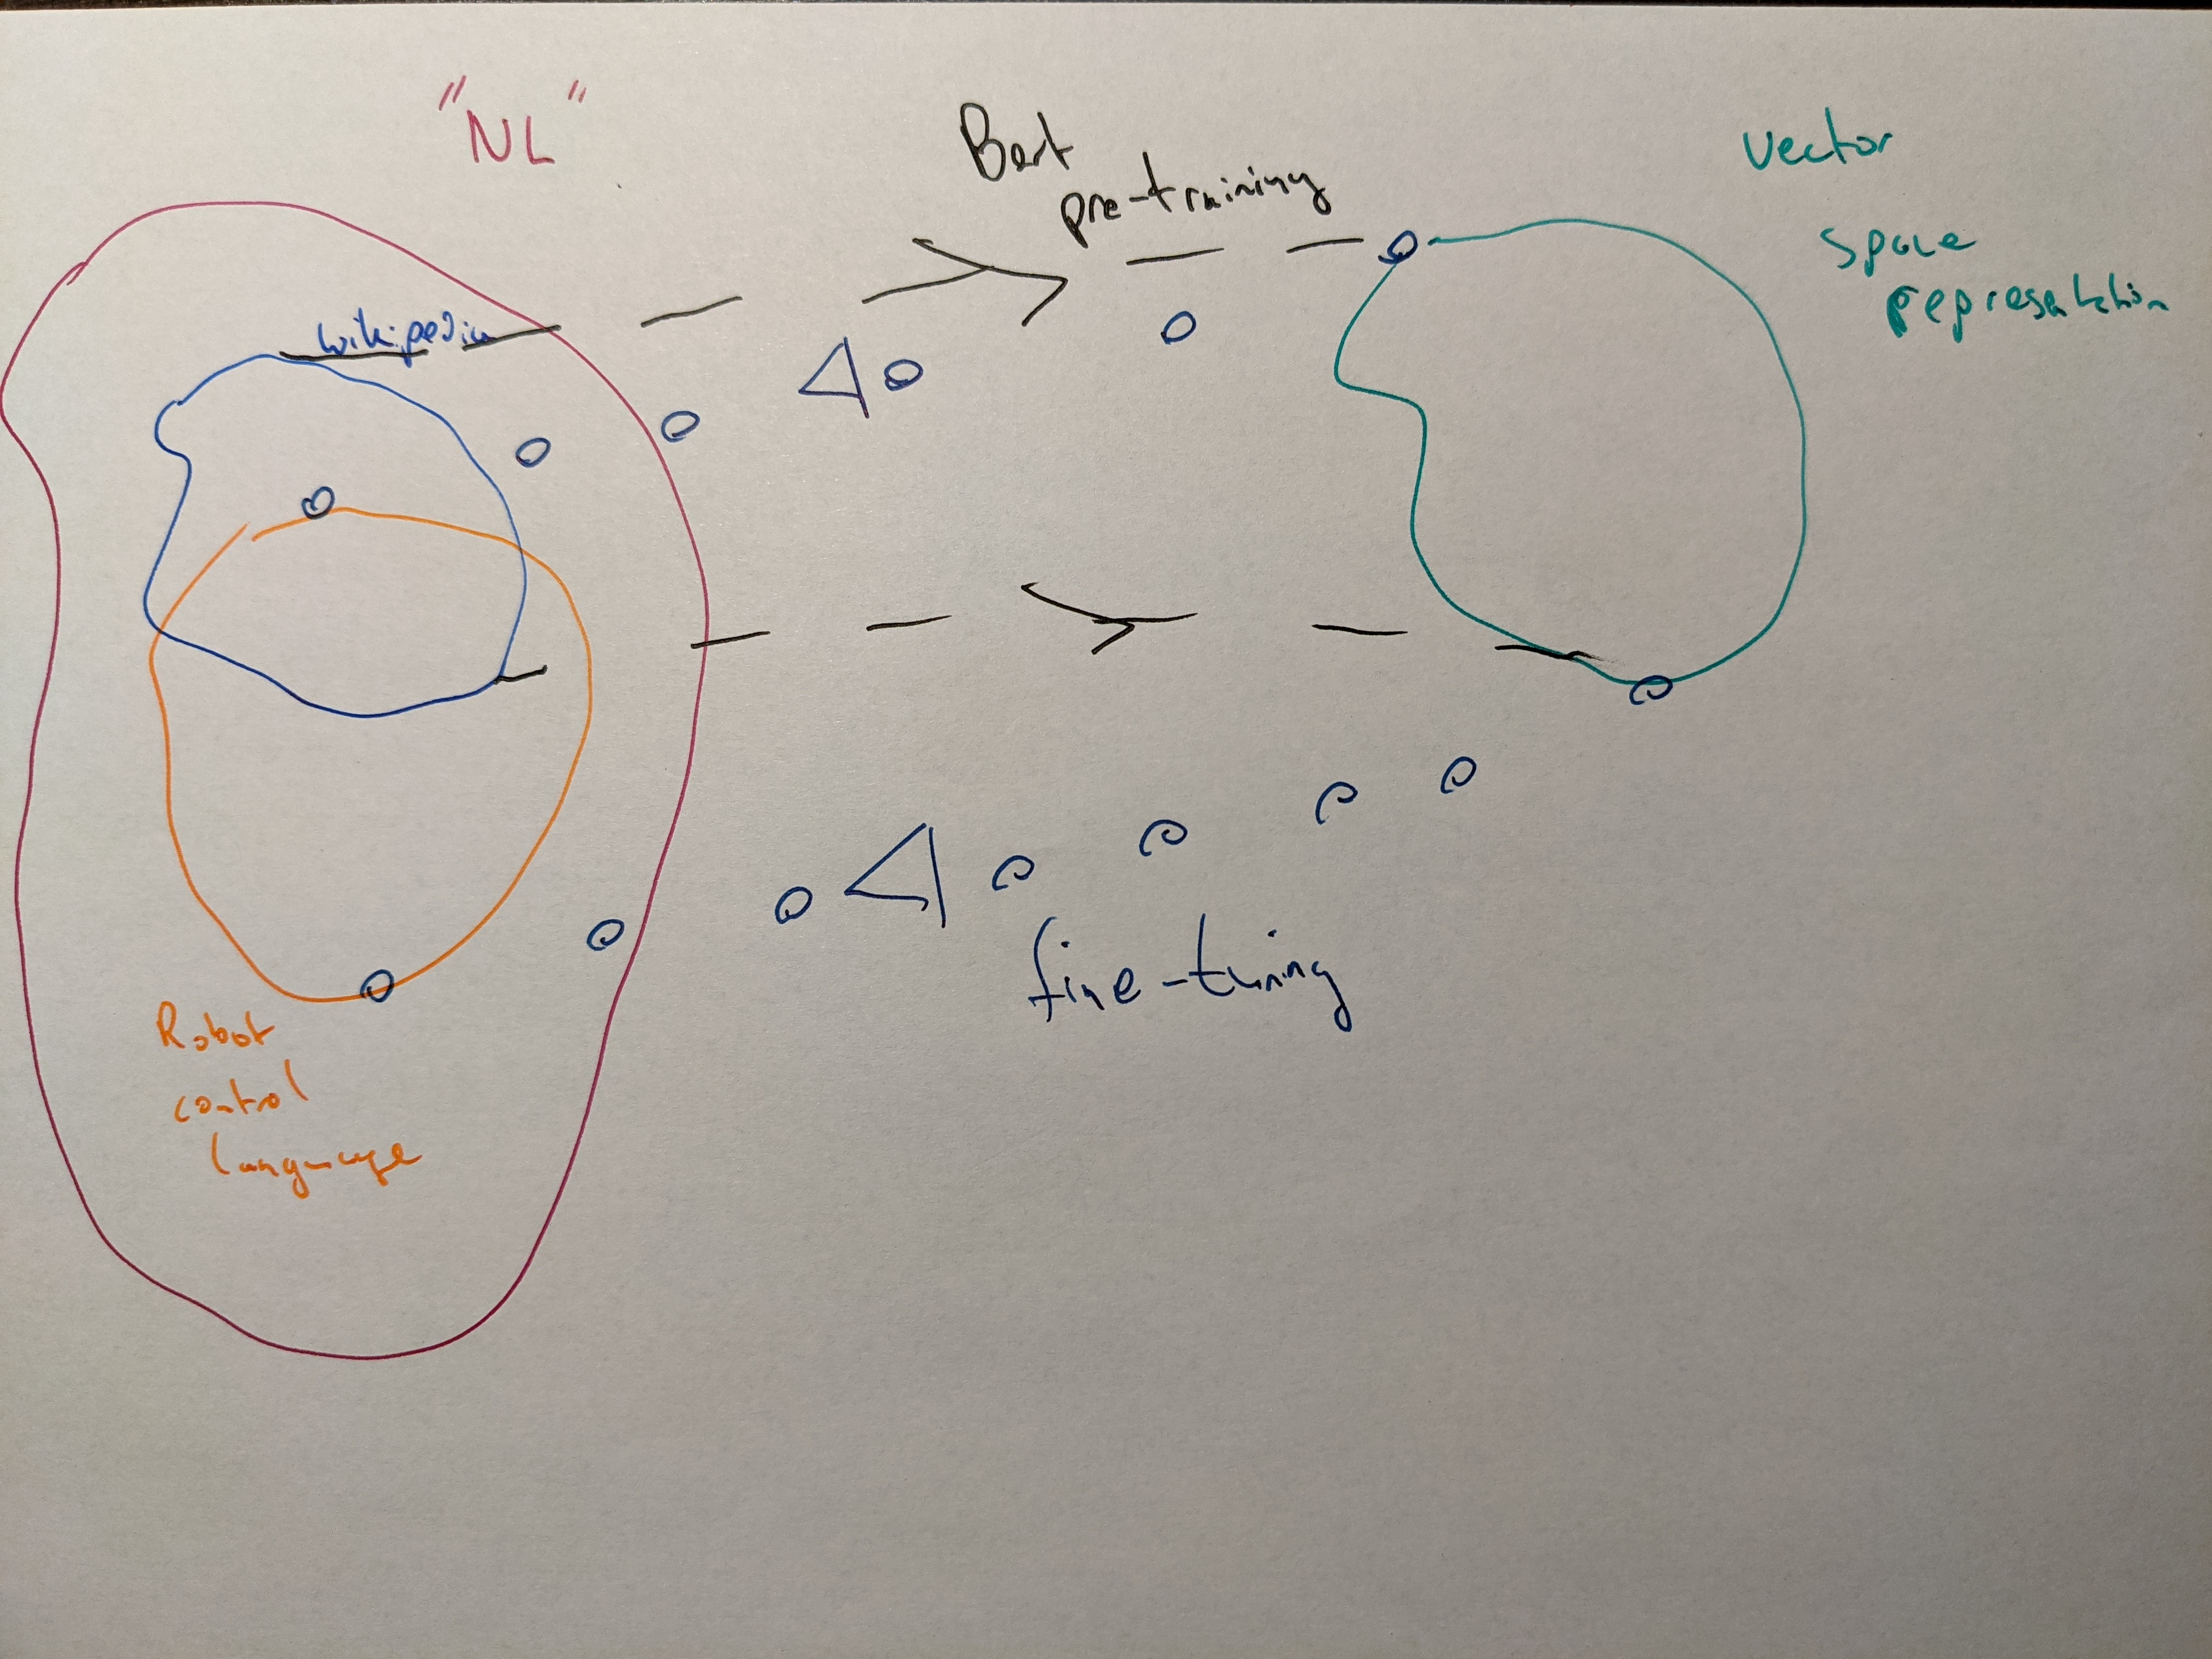
\includegraphics[width= \paperwidth]{pics/two.jpg}
\end{figure}
\end{frame}


\begin{frame}
\frametitle{}
\begin{figure}
\hspace*{-3mm}%
   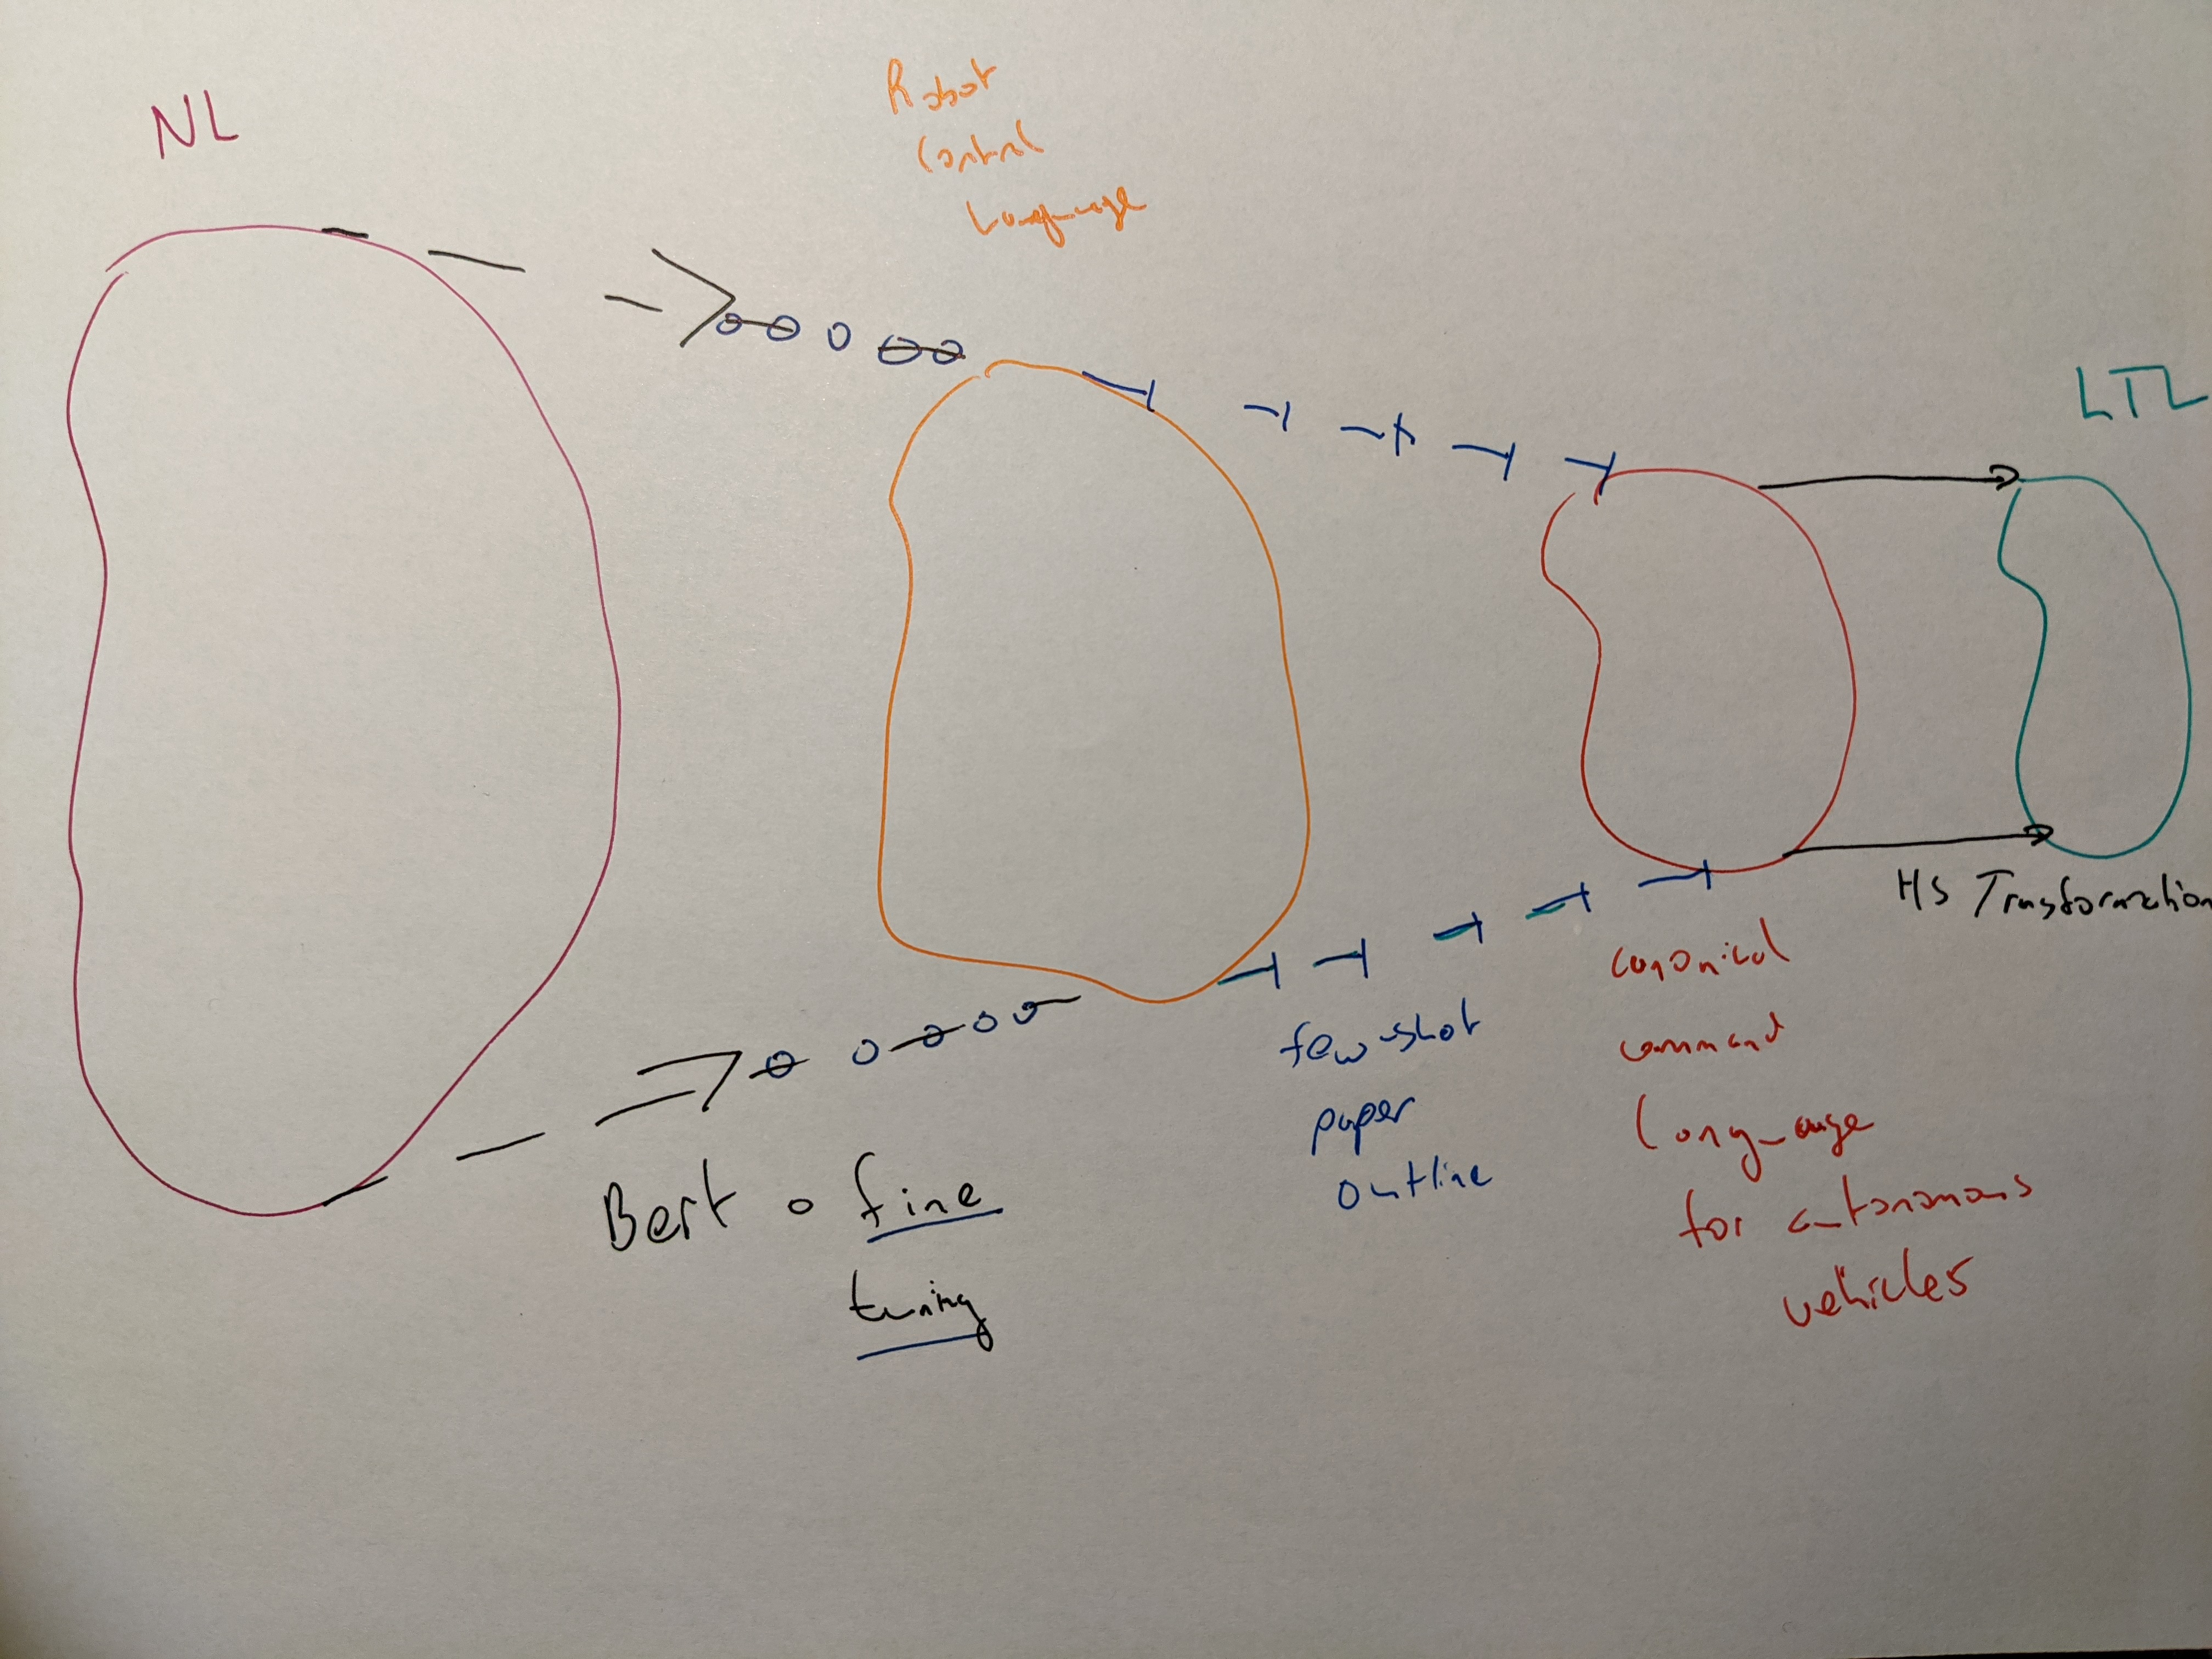
\includegraphics[width= \paperwidth]{pics/three.jpg}
\end{figure}
\end{frame}

\begin{frame}
\frametitle{Future}

\begin{itemize} 
\item Expand parser itself
\item Work on semantics , more expressive logic, etc
\item Ground semantics to Touchdown location map
\item Better data set?
\item Working on a draft document, with references, of everything shown here.
\end{itemize} 

\end{frame}

\end{document}
